%% Copernicus Publications Manuscript Preparation Template for LaTeX Submissions
%% ---------------------------------
%% This template should be used for copernicus.cls
%% The class file and some style files are bundled in the Copernicus Latex Package which can be downloaded from the different journal webpages.
%% For further assistance please contact the Copernicus Publications at: publications@copernicus.org
%% http://publications.copernicus.org


%% Please use the following documentclass and Journal Abbreviations for Discussion Papers and Final Revised Papers.


%% 2-Column Papers and Discussion Papers
\documentclass[gmd, manuscript]{copernicus}



%% Journal Abbreviations (Please use the same)

% Atmospheric Chemistry and Physics (acp)
% Advances in Geosciences (adgeo)
% Advances in Statistical Climatology, Meteorology and Oceanography (ascmo)
% Annales Geophysicae (angeo)
% ASTRA Proceedings (ap)
% Atmospheric Measurement Techniques (amt)
% Advances in Radio Science (ars)
% Advances in Science and Research (asr)
% Biogeosciences (bg)
% Climate of the Past (cp)
% Drinking Water Engineering and Science (dwes)
% Earth System Dynamics (esd)
% Earth Surface Dynamics (esurf)
% Earth System Science Data (essd)
% Fossil Record (fr)
% Geographica Helvetica (gh)
% Geoscientific Instrumentation, Methods and Data Systems (gi)
% Geoscientific Model Development (gmd)
% Geothermal Energy Science (gtes)
% Hydrology and Earth System Sciences (hess)
% History of Geo- and Space Sciences (hgss)
% Journal of Sensors and Sensor Systems (jsss)
% Mechanical Sciences (ms)
% Natural Hazards and Earth System Sciences (nhess)
% Nonlinear Processes in Geophysics (npg)
% Ocean Science (os)
% Primate Biology (pb)
% Scientific Drilling (sd)
% SOIL (soil)
% Solid Earth (se)
% The Cryosphere (tc)
% Web Ecology (we)


\begin{document}

\linenumbers

\title{An automatic and effective parameter optimization method for model tuning}


% % \Author[affil]{given_name}{surname}

\Author[1,2]{Tao}{Zhang}
\Author[3]{Lijuan}{Li}
\Author[2]{Yanluan}{Lin}
\Author[1,2]{Wei}{Xue}
\Author[1]{Haoyu}{Xu}
\Author[3]{Feng}{Xie}
\Author[1]{Xin}{Huang}

\affil[1]{Department of Computer Science and Technology, Tsinghua University, Beijing 100084}
\affil[2]{Center for Earth System Science, Ministry of Education Key Laboratory for Earth System Modeling, Tsinghua University, Beijing 100084}
\affil[3]{State Key Laboratory of Numerical Modeling for Atmospheric Sciences and Geophysical Fluid Dynamics, Institute of Atmospheric Physics, Chinese Academy of Sciences, Beijing 100029}

% %% The [] brackets identify the author with the corresponding affiliation. 1, 2, 3, etc. should be inserted.


\runningtitle{TEXT}

\runningauthor{TEXT}

\correspondence{Wei Xue (xuewei@tsinghua.edu.cn) }



% \received{}
% \pubdiscuss{} %% only important for two-stage journals
% \revised{}
% \accepted{}
% \published{}

% %% These dates will be inserted by Copernicus Publications during the typesetting process.


% \firstpage{1}

\maketitle
 

\begin{abstract}  

Physical parameterizations in General Circulation Models (GCMs), having various uncertain parameters, greatly impact model performance and model climate sensitivity.  Traditional manual and empirical tuning of these parameters is time consuming and ineffective. In this study, a ``three-step'' methodology is proposed to automatically and effectively obtain the optimum combination of some key parameters in cloud and convective parameterizations according to a comprehensive objective evaluation metrics. Different from the traditional optimization methods, two extra steps, one determines parameter sensitivity and the other chooses the optimum initial value of sensitive parameters, are applied before the downhill  simplex method to reduce the computational cost and improve the tuning performance. Atmospheric GCM simulation results show that the optimum combination of these parameters determined using this method is able to improve the model’s overall performance by 9\%. The proposed methodology and software framework can be easily applied to other GCMs to speed up the model development process, especially regarding unavoidable comprehensive parameters tuning during the model development stage. 

\end{abstract}


\introduction  %% \introduction[modified heading if necessary] 

Due to their current relatively low model resolutions, General Circulation Models (GCMs) need to parameterize various sub-grid scale processes. However, due to the complexities involved in these processes, parameterizations representing sub-grid scale physical processes unavoidably involve some empirical or statistical parameters \citep{hack1994climate}, especially within cloud and convective parameterizations. Physical parameterizations aim to approximate the overall statistical outcomes of various sub-grid scale physics \citep{williams2005modelling}. Consequently, these parameterizations introduce uncertainties to climate simulations using climate system models \citep{warren1979seasonal}. In general, these uncertain parameters need to be calibrated or constrained when new parameterization schemes are developed and integrated into models \citep{li2013evaluation}.


Traditionally, the uncertain parameters are manually tuned by comprehensive comparisons of model simulations with available observations. Such an approach is subjective, labor intensive, and hard to be extended \citep{hakkarainen2012closure, allen2000quantifying}. By contrast, the automatic parameter calibration techniques have progressed quickly because of their efficiency, effectiveness and broader applications \citep{emi2013collaborative,elkinton2008algorithms,jakumeit2005parameter,chen1999optimum}. In previous studies of their applying to GCMs, the methods can be categorized into three major types based on probability distribution function (PDF) method, optimization algorithms, and data assimilation techniques. 


For the PDF method, the confidence range of the optimization parameters is evaluated based on likelihood and Bayesian estimation. \cite{cameron1999flood} improves the forecast by the generalized likelihood uncertainty estimation (GLUE) \citep{beven1992future}, a method obtaining parameters uncertain range of a specific confidence level. The Bayesian Markov Chain Monte Carlo (MCMC) \citep{gilks2005markov} is widely used to obtain posterior probability distributions from prior knowledge. A couple of specific algorithms based on the MCMC theory are used to calibrate models in the previous literatures, such as Metropolis-Hasting \cite{sun2013inverse} adaptive Metropolis (AM) algorithm \cite{hararuk2014evaluation}, and. multiple very fast simulated annealing (MVFSA)\cite{jackson2008error} .The MVFSA method is one to two orders of magnitude faster than the Metropolis-Hasting algorithm \citep{jackson2004efficient}. However, these methods only attempt to determine the most likely area and cannot directly give the best combination of uncertain parameters with a minimum metrics value. Moreover, the posterior distribution heavily depends on the likelihood function assumed, which is usually difficult to determine for climate system model tuning problem.


Optimization algorithms can be used to search the maximum or minimum metrics value in a given parametric space. \cite{severijns2005optimizing} calibrates parameters of radiation, clouds, and convection in Speedy with downhill simplex \citep{press1992numerical, nelder1965simplex} to improve the radiation budget at the top of the atmosphere and at the surface, as well as the large scale circulation. Downhill simplex is a fast convergence algorithm when the parametric space is not high. However, it is a local optimization algorithm, not aiming to find the global optimal solution. Meanwhile, the algorithm has convergence issue when the simplex becomes ill-conditioned. Besides downhill simplex, a few global optimization algorithms are introduced to tune uncertain parameters of climate system models, such as simulated stochastic approximation annealing (SSRR) \cite{yang2013uncertainty}, MVFSA \cite{yang2014calibration} ,and multi-objective particle swarm optimization (MOPSO) \cite{gill2006multiobjective} . SSRR requires at least ten thousands of steps to get a stable solution \citep{liang2013simulated}, and MVFSA also requires thousands of steps \citep{jackson2004efficient}. MOPSO needs dozens of individual cases in each iteration. All these global optimization algorithms lead to large number of model runs and very high computational cost during the model tuning process.


Data assimilation method has been well addressed for state estimation, which is also regarded as a potential solution for parameter estimation. \cite{aksoy2006ensemble} estimates the parameter uncertainty of the NCAR/PSU Mesoscale
Model version 5 (MM5) \citep{haagenson1994penn} using the Ensemble Kalman Filter (ENKF). \cite{santiti2013simulated} presents a two-step filtering for the joint state-parameter estimation with a combination method of particle filtering (PF) and ENKF.  ENKF and PF have the difficulty in looking for the representative samples. Moreover, same as the MOPSO method, they require a large number of individual samples in each iteration with greatly increased computational resources.


Climate system model is a strongly nonlinear system, having large number of uncertain parameters. As a result, the parameter space of a climate system model is high-dimensional, multi-modal, strongly nonlinear, unseparable. The above mentioned methods generally require long iterations for convergence. More seriously, one sample run of a climate system model might require tens or even hundreds years of simulation to get scientifically meaningful results.


To overcome these challenges, we propose a ``three-step'' strategy to  calibrate the uncertain parameters in climate system models effectively and efficiently. First, a global sensitivity analysis method, Morris \citep{morris1991factorial, campolongo2007effective}, is chosen to eliminate the insensitive parameters by analyzing the main and interaction effects among parameters. Another global method by Sobol \citep{sobol2001global} is used to validate the results of Morris. Second, a pre-processing of initial values of parameters is presented to accelerate the optimization and to resolve the issue of ill-conditioned simplex. Finally, the downhill simplex algorithm is used to solve the optimization problem because of its low computational cost and fast convergence for the low dimension parameter problem. Taking into account the complex configuration and manipulation of model tuning, an automatic workflow is designed and implemented to make the calibration process more efficient. This is result already. The method and workflow can be easily applied to GCMs to speed up model development process.


The paper is organized as follows. Section 2 introduces the automatic workflow proposed. Section 3 describes the details of GAMIL2, reference data, and calibration metrics. The three-step calibration strategy is presented in Section 4. Section 5 evaluates the calibration results, followed by a summary and discussion in Section 6.


\section{The end-to-end automatic calibration workflow}

We designed a software framework for the overall control of the tuning practice. It incorporates various tuning methods and facilitate model tuning process with minimal manual management. It effectively manages the dependence and calling sequences of various procedures, including parameter sampling, sensitivity analysis and initial value selection, model configuration and running, simulation evaluation using user provided reference metrics. Users only need to specify the model to tune, parameters to be tuned with their valid ranges, and the calibration method to use. The workflow is designed to automatically execute any part of the ``three-step'' calibration strategy, and determine the optimal parameters and its corresponding diagnostic results. 

There are four main modules within the framework. The task scheduler module manages model simulations with the capability for simultaneous runs. It also coordinates different tasks to reduce the contention and improve throughput. Simulation diagnosis and evaluation is included in a post-processing module.  The preparation module contains various sensitivity analysis and sampling methods, such as Morris and Sobol, full factorial(FF) \citep{raktoe1981factorial}, Latin Hypercube (LH) \citep{mckay1979comparison}, Morris one-at-a-time (MOAT) \citep{morris1991factorial}, and Central Composite Designs (CCD) \citep{hader1978slope}. The sensitivity analysis is able to eliminate the duplicated samples to reduce unnecessary computing loads. A MCMC method based on adaptive Metropolis-Hastings algorithms is also provided to get the posterior distribution of uncertain parameters. The calibration module offers various local and global optimization algorithms including the downhill simplex, genetic algorithm, particle swarm optimization, differential evolution and simulated annealing. In addition, all the intermediate metrics and their corresponding parameters within the framework are stored in a MySQL database and can be used for posterior knowledge analysis. More importantly, the workflow is flexible and expandable for easy integration of other advanced algorithms as well as tools like the Problem Solving Environment for Uncertainty Analysis and Design Exploration (PSUADE) \citep{tong2005psuade}, Design Analysis Kit for Optimization and Terascale Applications (DAKOTA) \citep{eldred2007investigation}. Although, uncertainty quantification toolkits, such as PSUADE, DAKOTA, support various calibration and uncertainty analysis methods and pre-defined function interfaces,  they cannot organize the above model tuning process effectively.


\section{Model description and reference metrics}
We use the Grid-point Atmospheric Model of IAP LASG version 2 (GAMIL2) as an example for the demonstration of the method. GAMIL2 is the atmospheric component of the Flexible Global-Ocean-Atmosphere-Land System Model grid version 2 (FGOALS-g2), which participated in the CMIP5 program. The horizontal resolution is 2.8 x 2.8 degree, with 26 vertical levels. GAMIL2 uses a finite difference scheme that conserves mass and energy \citep{wang2004design}. A two-step shape-preserving advection scheme \citep{rucong1994two} is used for tracer advection. Compared to the pervious version, GAMIL2 has modifications in cloud-related processes \citep{li2013evaluation}, such as the deep convection parameterization \citep{zhang2005effects}, the convective cloud fraction \citep{xu1991evaluation}, and the cloud microphysics \citep{morrison2008new}. More details are in \cite{li2013evaluation}. Empirical tunable parameters are selected  from schemes of deep convection, shallow convection, and cloud fraction schemes (Table 1). Default parameter values are the configuration for the standard version used for CMIP5 experiments.

To save computational cost, atmosphere-only simulations are conducted for 5 years using prescribed seasonal climatology (no interannual variation) of SST and sea ice. Previous studies have shown 5 years of this type of simulation is enough to capture some basic model characteristics. The goal of these sensitivity simulations is not to determine their resemblance to observations, but to compare the results between the control simulation and various tuned simulations.

Model tuning results depend on the reference metrics used. For a simple justification, we use some conventional climate variables for the evaluation. Wind, humidity, and geopotential height are from the European Center for Medium-Range Weather Forecasts (ECMWF) Re-Analysis (ERA) - Interim reanalysis from 1989 to 2004 \citep{simmons2007era}. We use GPCP (Global Precipitation Climatology Project, \citep{adler2003version}) for precipitation and ERBE (Earth Radiation Budget Experiment, \citep{barkstrom1984earth}) for radiative fields. All observational and reanalysis data are gridded to the same grid as GAMIL2 before the comparison. Note that the evaluation metrics can be extended depending on the model performance requirement. 


A comprehensive metrics, including various variables in Table 2, is used to quantitatively evaluate the performance of overall simulation skills \citep{murphy2004quantification, gleckler2008performance, reichler2008well}. The calibration RMSE is defined as the spatial standard deviation (SD) of the model simulation against observations/re-analysis, as in Eq. 1 \citep{taylor2001summarizing,yang2013uncertainty}. For an easy comparison, we normalize the RMSE of each simulation by that of the control simulation. We weight each variable equally and compute the average normalized RMSE, which indicates the overall improvement relative to the control simulation if it is less than 1. 


\begin{align}
(\sigma_m^F)^2 &= \sum_{i=1}^l w(i)(x_m^F(i) - x_o^F(i))^2 \\
(\sigma_r^F)^2 &= \sum_{i=1}^l w(i)(x_r^F(i) - x_o^F(i))^2 \\
\chi^2 &= \frac{1}{N^F}\sum_{F=1}^{N^F} (\frac{\sigma_m^F}{\sigma_r^F})^2
\end{align}

$x_m^F(i)$ is the model outputs according to selected shown in the Table 2. $x_o^F(i)$ is the 
corresponding observation or reanalysis data. $x_r^F(i)$ is the reference results from CMIP5. w is 
the weight due to the different grid area. I is the total grid number in model. $N^F$ is the 
number of the chosen variables.


\section{Method}
\subsection{Global and local optimization method} 
Parameter tuning for a climate system model is to solve a global optimization problem in theory.  However, traditional evolutionary algorithms, such as genetic algorithm \citep{goldberg1989messy}, differential evolutionary (DE) \citep{storn1995differential}, and particle swarm optimization (PSO) \citep{kennedy2010particle}, generally require at least  thousands of iterations to get a stable global solution and need to set a population of individuals in each iteration, leading to high computational cost \citep{hegerty2009comparative,shi1999empirical}. Model tuning is always a trade-off between performance and computational cost. Therefore, it is critical to get the best possible results with limited numbers of simulations. In this sense, local optimization algorithms are the viable options  considering their significantly reduced computational cost.


We choose the downhill simplex method for climate model tuning considering its relatively low computation cost. Downhill simplex searches the optimal solution by changing the shape of a simplex, which represents the optimal direction and step length. A simplex is a geometry, consisting of $N+1$ vertexes and their interconnecting edges, where \textit{N} is the number of calibration parameters. The vertexes stand for the pair of a set of parameters and their metrics. The new vertex is determined by expanding and shrinking the vertex with the highest metrics value, leading to a new simplex \cite{press1992numerical} and \cite{nelder1965simplex}.


For example, global PSO and DE method give better tuning results compared to the local downhill simplex method, but their computational costs are approximately 4 and 5 times of the downhill simplex method, respectively (Table 3). 


To improve the effectiveness and performance of the local downhill simplex method, we propose two important steps to significantly improve its performance. In the first step, the number of tuning parameters is reduced by eliminating the insensitive parameters; In the second step, fast convergence for better solution is achieved by pre-selecting proper initial values before downhill simplex method.

\subsection{Parameter sensitivity analysis}

The number of uncertain parameters in physical parameterizations of the climate system model is quite large. Most optimization algorithms, such as PSO, downhill simplex, and simulated annealing algorithm \citep{van1987simulated}, are ineffective in high dimension problems. Iterations for convergence will increase exponentially with the parameters need to be tuned.  In addition, climate models generally need a long simulation to have meaningful results. Therefore, solving high dimension parameter tuning problem suffers from extreme calibration computational cost.  Thus, it is necessary to reduce the parameters dimension before the optimization.

The sensitivity analysis can be divided into local and global method \citep{gan2014comprehensive}. The local method only gets the main effect of a parameter by perturbing one parameter value. The linear correlation coefficient can only measure the linear sensitivity, but it cannot present the nonlinear sensitivity. The Morris method \citep{morris1991factorial, campolongo2007effective} is a qualitative global sensitivity method. The advantage of this method is that not only the single parameter sensitivity can be calculated, but also the interactive sensitivity among parameters can be known at the same time.


The sampling strategy is based on MOAT experimental design with relatively less samples required. It only needs $(n+1) \times M$ samples, where \textit{n} is the number of calibration parameters and \textit{M} is the number of trajectories, usually from 10 to 20. Considering the \textit{n} parameters $x_i (i=1,...,n)$, normalized to [0,1], the influence of each variable is defined as an elementary effect, shown as Eq. 4, where $\Delta$ is the step size for each parameter. The starting point of a trajectory is selected randomly and the next point is chosen by changing one unchanged parameter value at one time in a random order until getting $n+1$ samples. The mean of $|d_j|$ stands for the main effect of a single parameter, and the standard deviation presents the interactive effect among multiple parameters. Therefore, those parameters with a low mean and low standard deviation is regard as the insensitive ones for the metrics and will be eliminated during the following optimization step.


\begin{align}
& d_{ij} = \frac{y(X_1,...,X_j+\Delta,...,X_N)-y(X_1,...,X_j,...,X_N)}{\Delta} \\
& \mu_j = avg(|d_{i,j}|), \sigma_j = stddev(d_{i,j}) 
\end{align}

Taking GAMIL2 as an example, tunable parameters in Table 2 are required to perform sensitivity analysis. We perform 80 samples, and the results are shown in Figure 1. The insensitivity parameters, ke, capelmt, and c0 of shallow convection, will not be taken into consideration in the next step.


The parameter elimination step is critical for the final result of model tuning. To validate the results got by Morris, we compare the results with those with Sobol’s benchmark method \citep{sobol2001global}. It is also a quantitative method based on variance decomposition requiring more samples than the Morris, with a higher computation cost. The variance of the model output can be decomposed as equation (3), where \textit{n} is the number of parameters, and $V_i$ is the variance of the $i_{th}$ parameter, and $V_{ij}$ is the variance of the interactive effect between the  and $j_{th}$ parameters, and so on. The total sensitivity effect of $i_{th}$ parameter can be presented as equation (4), where $V_{-i}$ is the total variance except for the $x_i$ parameter. The Sobol results are shown as Figure 2.  The screened out parameters are the same ones as those of the Morris.

The parameter elimination step is critical for the final result of model tuning. To validate the results by Morris, we compare the results with those with Sobol’s benchmark method \citep{sobol2001global}. It is also a quantitative method based on variance decomposition requiring more samples than the Morris, with a higher computation cost. The variance of the model output can be decomposed as Eq. 6, where \textit{n} is the number of parameters, and $V_i$ is the variance of the $i_{th}$ parameter, and $V_{ij}$ is the variance of the interactive effect between the  and $j_{th}$ parameters, and so on. The total sensitivity effect of $i_{th}$ parameter can be presented as Eq. 7, where $V_{-i}$ is the total variance except for the $x_i$ parameter. The Sobol results are shown in Figure 2.  The screened out parameters are the same as those of the Morris.

\begin{align}
& V = \sum_{i=1}^n V_i + \sum_{1 \leq i < j \leq n} V_{ij} + ... + V_{1,2,...,n}  \\
& S_{T_i} = 1 - \frac{V_{-i}}{V} 
\end{align}


\subsection{Proper initial values selection of downhill simplex}

Since the downhill simplex method is a local optimization algorithm, its convergence performance strongly depends on the quality of the initial values. We need to find the parameter combinations with the smaller metrics around the final solution. Moreover, we have to complete the searching as fast as possible for minimal overhead. For these two objectives, a hierarchical sampling based on the full factor sample method is used. The method uses a longer distance to find the candidate regions for the optimal solution first followed by a second round sampling using a smaller distance to reduce the interested region. The simple sampling method is easy to implement and has lower overhead compared to other complex adaptive sampling methods.


At the same time, inappropriate initial values may lead to ill-conditioned simplex geometry, which can be found in model tuning. One issue we meet is that some parameters keep the same value as the initial value. As a result, these parameters are invariant during the optimization by using the downhill simplex method and this leads to poor performance of optimization. Consequently, simplex checking is conducted to keep as many as different parameters values during looking for initial values. Well-conditioned simplex geometry will increase the parameter freedom for optimization with faster convergence. This procedure is presented as the initial value pre-processing of the downhill simplex algorithm.


It is noted that samples for looking for initial values sometimes can be the same ones in dimension reduction step. In this case, one model run can be used in the two steps to further reduce computational cost.



\subsection{Evaluate the optimal strategy}

In table 3, PSO gets the best solution. But this global method spends more computational cost than the local downhill simplex method. Taking into account the bad effectiveness of downhill simplex, we present two other strategies, the proposed three-step, and a ``two-step'' method only including the initial value pre-processing and downhill simplex method . The downhill simplex in the three-step tunes the sensitive parameters described in section 2.1. The initial values pre-processing requires extra 25 sampling points, and the parameter sensitivity analysis with Morris requires 80 sampling points. In Table 4, the two-step gets a better solution than the ``one-step'' downhill simple. It indicates pre-selecting of the proper initial values can remarkably improve the calibration performance. Although the two-step method has the best efficiency, the solution is worse than the three-step method. Meanwhile, the computational cost of all strategies based on the local algorithm are smaller than that of the global method. With the results in Table 3 and Table 4, we can conclude that the proposed three-step method can achieve the best trade-off between accuracy and computational cost.


\section{Model improvement analysis}
This section compares the default simulation and the tuned simulation with a focus on the cloud and TOA radiation changes. Table 1 shows the values of the four pairs of sensitive parameters between the default (labeled as CNTL) and optimized simulation (labeled as EXP). Significant change is found for c0, which represents the auto-conversion coefficient in the deep convection scheme, and rhminh, which represents the threshold relative humidity for high cloud appearance. The other two parameters have negligible change of the values before and after the tuning and thus it is expected their impacts on model performance will be accordingly small.


The overall improvement after the tuning from the control simulation can be found in the Taylor diagram (Fig. 4), with improvement for almost all the variables, especially for the meridional winds and mid-tropospheric (400 hPa) humidity. Improvements for other variables are relatively small. The change in terms of the RMSE factor over the globe and three regions (tropics, SH mid- and high-latitude and NH mid- and high-latitude) are shown in Fig. 5. First, radiative fields and moisture are improved over all the four areas. By contrast, wind and temperature field changes are more diverse among different areas. This is partly due to the fact that the tuned parameters have direct impacts on moisture and cloud fields. While wind and temperature fields are indirectly influenced following the cloud and radiative impacts. For example, temperatures over the tropics become worse compared to the control run. There is an overall improvement in the SH mid- and high-latitude for all variables except for the 200 hPa temperature. Winds and precipitation in the NH mid- and high-latitude become slightly worse in the tuned simulation. Such changes are kind of intriguing and we attempt to relate these changes to the two parameters significantly tuned.


With increased auto-conversion coefficient in the deep convection, less condensate is detrained to the environment. As a result, mid- and upper-troposphere is overall drier, especially over the tropics where deep convection dominates the vertical transport of water vapor (Fig. 6a).  Although the mid- and upper-troposphere become drier over the tropics, reduced RH threshold for high cloud makes clouds easier to be present. Consequently, middle and high clouds increase over the globe, especially over the mid- and high-latitudes with the largest increase up to 4-5\%. In the tropics, due to the drier tendency induced by the reduced detrainment, high cloud increase is relatively small (2-3\%) compared to the mid- and high- latitudes. Below ~800 hPa, low clouds decrease by 2-3\% over the mid- and high-latitudes. The reason for this low cloud reduction is still under investigation. 


Changes in moisture and cloud fields impact radiative fields.  With reference to ERBE, TOA outgoing longwave radiation (OLR) is improved in the mid-latitudes for EXP, but it is degraded over the tropics (Fig. 7a). Compared with the CNTL, middle and high cloud significantly increase in the EXP (Fig. 6). Consequently, it enhances the blocking effect on the longwave upward flux at TOA (FLUT), reducing the FLUT in mid-latitudes of the southern and northern hemisphere (Fig. 8a). Clear sky OLR increases for the EXP and this is due to the drier upper troposphere in the EXP (Fig. 6). The decrease in the atmospheric water vapor reduces the greenhouse effect. Therefore, it emits more outgoing longwave radiation and reduces the negative bias of clear sky long wave upward flux at TOA (FLUTC, Fig. 8b). Longwave cloud forcing (LWCF) in the middle and high latitudes is improved due to the improvement of FLUT in this area (Fig. 8c), but improvement in the tropics is negligible due to the cancellation between the FLUT and FLUTC. 


TOA clear sky shortwave are the same between the control and the tuned simulation since both simulation has the same surface albedo. With increased clouds, the tuned simulation has smaller TOA shortwave absorbed than the control. Compared with ERBE, the tuned simulation has better TOA shortwave absorbed in the mid- and high-latitudes, but it slightly degrades over the tropics.  



\conclusions  %% \conclusions[modified heading if necessary]  

An effective and efficient three-step method for GCM physical parameter tuning is proposed. Compared with conventional methods, an insensitive parameter reduction step and a proper initial value selection step are applied before the local optimization method. This effectively reduces the computational cost with an overall good performance.    In addition, an automatic parameter calibration workflow is designed and implemented to enhance operational efficiency and to support multiple uncertainty quantification analysis and calibration strategies. testing of the method using the GAMIL2 model indicates the three-step outperforms the two global optimization methods (PSO and DE) in both effectiveness and efficiency.  A better trade-off between accuracy and computational cost is achieved compared with the two-step method and the downhill simplex method. The optimal results of the three-step method demonstrate that most of the variables are improved compared with the control experiment, especially for the radiation related variables. The mechanism analysis are conducted to explain why these radiation related variables have an overall improvement.

Recently, the surrogate-based optimization method has been an active research area . The idea is to  approximate the real models by  statistical regression methods to greatly reduce the computational cost. However, the precision of surrogate models cannot meet the requirement for the strong non-linear climate system model, especially for wind fields. Therefore, it is also worth to continue improving the calibration strategies based on real models. We plan to evaluate the computationally-cheap surrogate model, further reducing the computational cost for calibrating the climate system model. In addition, more analyses are needed to better understand the model behavior changes.

 
% \appendix
% \section{}    %% Appendix A

% \subsection{}                               %% Appendix A1, A2, etc.




% \begin{acknowledgements}
% TEXT
% \end{acknowledgements}


% %% REFERENCES

% %% The reference list is compiled as follows:

% %\begin{thebibliography}{}

% %\bibitem[AUTHOR(YEAR)]{LABEL}
% %REFERENCE 1
% %
% %\bibitem[AUTHOR(YEAR)]{LABEL}
% %REFERENCE 2
% %
% %\end{thebibliography}

% %% Since the Copernicus LaTeX package includes the BibTeX style file copernicus.bst,
% %% authors experienced with BibTeX only have to include the following two lines:
% %%
\bibliographystyle{copernicus}
\bibliography{uq}
%%
%% URLs and DOIs can be entered in your BibTeX file as:
%%
%% URL = {http://www.xyz.org/~jones/idx_g.htm}
%% DOI = {10.5194/xyz}


%% LITERATURE CITATIONS
%%
%% command                        & example result
%% \citet{jones90}|               & Jones et al. (1990)
%% \citep{jones90}|               & (Jones et al., 1990)
%% \citep{jones90,jones93}|       & (Jones et al., 1990, 1993)
%% \citep[p.~32]{jones90}|        & (Jones et al., 1990, p.~32)
%% \citep[e.g.,][]{jones90}|      & (e.g., Jones et al., 1990)
%% \citep[e.g.,][p.~32]{jones90}| & (e.g., Jones et al., 1990, p.~32)
%% \citeauthor{jones90}|          & Jones et al.
%% \citeyear{jones90}|            & 1990

\clearpage
%% FIGURES

%% ONE-COLUMN FIGURES

%f
\begin{figure}[t]
\includegraphics[width=15.3cm]{workflow}
\caption{The structure of the automatic calibration workflow.The input of the workflow is the parameters of interest and their initial value range. The
output is the optimal parameters and its corresponding diagnostic results after calibrating with a calibration strategy. The preparation module provides the parameter sensitivity analysis. The calibration algorithm module offers local and global optimization algorithms including downhill simplex, genetic algorithm, particle swarm optimization, differential evolution and simulated annealing. The scheduler module schedules as many as cases to run simultaneously and coordinates the different tasks. The post-processing module is responsible for metrics diagnostics, re-analysis and observational data management.}
\end{figure}

\begin{figure}[t]
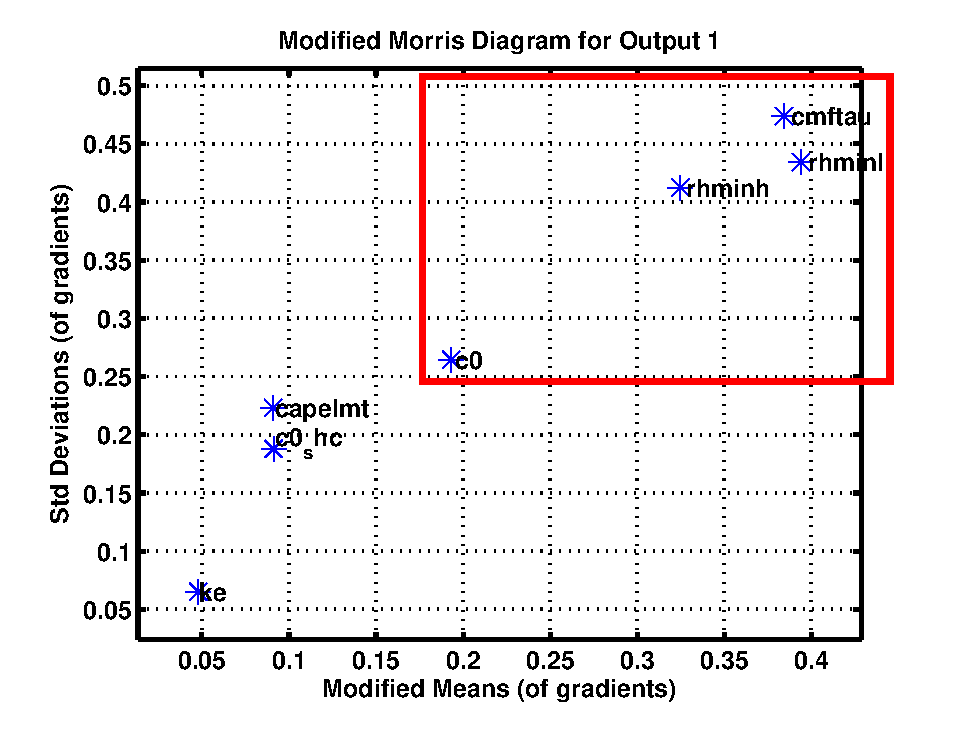
\includegraphics[width=8.3cm]{Morris}
\caption{Scatter diagram of Morris sensitivity analysis. The X-axis stands for the main effect sensitivity of single parameter. The Y-axis stands for the interactive effect among multi-parameters. Therefore, c0, rhminl, rhminh, and cmftau have high sensitivity. ke, c0\_shc, and capelmt have low sensitivity.}
\end{figure}

\begin{figure}[t]
\includegraphics[width=8.3cm]{Sobol}
\caption{Sobol sensitivity results. The total sensitivity in equation (7) is presented by the size of color area. The total sensitivities of ke, c0\_shc, and capelmt are not more than 0.5 with regard to each variable. They are insensitive.}
\end{figure}

\begin{figure}[t]
\includegraphics[width=12cm]{taylor}
\caption{Taylor diagram of the climate mean state of each variable from 2002 to 2004 of EXP and CNTL.}
\end{figure}

\begin{figure}[t]
\includegraphics[width=15.3cm]{reg}
\caption{The EXP metrics of each variable with the global, tropical, and northern/southern mid- and high-latitude.}
\end{figure}

\begin{figure}[t]
\includegraphics[width=15.3cm]{cloud-rh}
\caption{Pressure--latitude distributions of relative humidity and cloud fraction of EXP (a,d), CNTL (b,e), EXP-CNTL (c,f).}
\end{figure}

% \begin{figure}[t]
% \includegraphics[width=15.3cm]{cloud}
% \caption{Pressure--latitude distributions of cloud fraction of EXP (a), CNTL (b), and EXP-CNTL (c).}
% \end{figure}

\begin{figure}[t]
\includegraphics[width=12cm]{radiation-curve}
\caption{Meridional distributions of the annual mean difference between EXP/CNTL and observations of FLUT (a), FLUTC (b), LWCF (c), SWCF (d), FNSTOA(d), FNSTOAC(e), and SWCF(f).}
\end{figure}

\clearpage
%% TWO-COLUMN FIGURES

%f
%\begin{figure*}[t]
%\includegraphics[width=12cm]{FILE NAME}
%\caption{TEXT}
%\end{figure*}


%% TABLES
%%
%% The different columns must be seperated with a & command and should
%% end with \\ to identify the column brake.

%% ONE-COLUMN TABLE

%t

\begin{table}[t]
\caption{Initial selected uncertain parameters in GAMIL2 and their optimal values in EXP.}
\begin{tabular}{l l l c l}
\tophline
Parameter & Description & Default & Range & Optimal \\
\middlehline
c0 & rain water autoconversion coefficient for deep convection & 3.0e-4 & 1.e-4 $\sim$ 5.4e-3 & 5.427294e-4\\
ke & evaporation efficiency for deep convection & 7.5e-6 & 5e-7 $\sim$ 5e-5 & --\\
capelmt & threshold value for cape for deep convection & 80 & 20 $\sim$ 200 & --\\
rhminl & threshold RH for low clouds & 0.915 & 0.8 $\sim$ 0.95 & 0.917661 \\
rhminh & threshold RH for high clouds & 0.78 & 0.6 $\sim$ 0.9 & 0.6289215\\
c0\_shc & rain water autoconversion coefficient for shallow convection & 5e-5 & 3e-5 $\sim$ 2e-4 & -- \\
cmftau & characteristic adjustment time scale of shallow cape & 7200 & 900 $\sim$ 14400 & 7198.048 \\
\bottomhline
\end{tabular}
\belowtable{} % Table Footnotes
\end{table}

\begin{table}[t]
\caption{Model output variables and evaluation data in the metrics.}
\begin{tabular}{l l l l}
\tophline
Variable & Observation & Variable & Observation \\
\middlehline
Meridional wind at 850hPa   & ECMWF & Geopotential Z at 500hPa              & ECMWF \\
Meridional wind at 200hPa   & ECMWF & Total precipitation rate              & GPCP \\
Zonal wind at 850hPa        & ECMWF & Long-wave cloud forcing                & ERBE \\
Zonal wind at 200hPa        & ECMWF & Short-wave cloud forcing               & ERBE \\
Temperature at 850hPa       & ECMWF & Long-wave upward flux at TOA          & ERBE \\
Temperature at 200hPa       & ECMWF & Clearsky long-wave upward flux at TOA & ERBE \\
Specific Humidity at 850hPa & ECMWF & Short-wave net flux at TOA            & ERBE \\
Specific Humidity at 400hPa & ECMWF & Clearsky short-wave net flux at TOA   & ERBE \\
\bottomhline
\end{tabular}
\belowtable{} % Table Footnotes
\end{table}

% \begin{table}[t]
% \caption{Fall factor samplings of parameters and metrics.}
% \begin{tabular}{l l l l l l l l l l l l}
% \tophline
% ID & c0 & rhminl & rhminh & cmftau & metrics & ID & c0 & rhminl & rhminh & cmftau & metrics \\
% \middlehline
% 1  & 3.00E-04 & 0.915 & 0.78 & 7200 & 1     & 12 & 3.00E-04 & 0.915 & 0.6   & 7200  & 1.00547 \\
% 2  & 3.04E-04 & 0.915 & 0.78 & 7200 & 1.054 & 13 & 3.00E-04 & 0.915 & 0.675 & 7200  & 1.027676\\
% 3  & 7.13E-04 & 0.915 & 0.78 & 7200 & 0.987 & 14 & 3.00E-04 & 0.915 & 0.75  & 7200  & 1.023358\\
% 4  & 1.12E-03 & 0.915 & 0.78 & 7200 & 1.04  & 15 & 3.00E-04 & 0.915 & 0.825 & 7200  & 1.028264\\
% 5  & 2.55E-03 & 0.915 & 0.78 & 7200 & 1.075 & 16 & 3.00E-04 & 0.915 & 0.9   & 7200  & 1.160479\\
% 6  & 5.00E-03 & 0.915 & 0.78 & 7200 & 1.09  & 17 & 3.00E-04 & 0.915 & 0.78  & 900   & 1.22922 \\
% 7  & 3.00E-04 & 0.8   & 0.78 & 7200 & 1.223 & 18 & 3.00E-04 & 0.915 & 0.78  & 4275  & 1.064064\\
% 8  & 3.00E-04 & 0.838 & 0.78 & 7200 & 1.054 & 19 & 3.00E-04 & 0.915 & 0.78  & 7650  & 1.004806\\
% 9  & 3.00E-04 & 0.875 & 0.78 & 7200 & 1.019 & 20 & 3.00E-04 & 0.915 & 0.78  & 11025 & 1.077167\\
% 10 & 3.00E-04 & 0.913 & 0.78 & 7200 & 1.007 & 21 & 3.00E-04 & 0.915 & 0.78  & 14400 & 1.148265\\
% 11 & 3.00E-04 & 0.95  & 0.78 & 7200 & 1.094 \\
% \bottomhline
% \end{tabular}
% \belowtable{} % Table Footnotes
% \end{table}

\begin{table}[t]
\caption{Comparison with local and global algorithms. Downhill simplex is a local method. We use ``Downhill\_1\_step'' represents it,  distinguished from some optimal strategies based on the downhill simplex. PSO and DE are the global method. Optimal solution is the final calibrating result. $N_{step}$ is the total numbers of calibrating iteration. $N_{size}$ is the size of population of the global algorithms. Core hours is computed by $N_{step} \times N_{size} \times$ numbers of process (30) $\times$ hours of 5-years simulation (6).}
\begin{tabular}{l l l l l}
\tophline
  & Optimal solution & $N_{step}$ & $N_{size}$ & Core hours \\
\middlehline
Downhill\_1\_step & 0.9585    & 80         & 1  & 14400 \\
PSO               & 0.911537  & 24         & 12 & 51840 \\
DE                & 0.942148  & 33         & 12 & 71280 \\
\bottomhline
\end{tabular}
\belowtable{} % Table Footnotes
\end{table}

\begin{table}[t]
\caption{Comparison with optimal strategies based on the downhill simplex. The initial values pre-process is applied to Downhill\_2\_steps and Downhill\_3\_steps with extra 25 samples. In the Downhill\_3\_steps, a step of parameter sensitivity process is conducted before the initial values pre-precess with extra 80 samples.}
\begin{tabular}{l l l l l}
\tophline
  & Optimal solution & $N_{step}$ & $N_{size}$ & Core hours \\
\middlehline
Downhill\_1\_step & 0.9585    & 80         & 1  & 14400 \\
Downhill\_2\_steps  & 0.9256899 & 25+34    &  1 & 10620 \\
Downhill\_3\_steps  & 0.9098545 & 80+25+50 &  1 & 27900 \\
\bottomhline
\end{tabular}
\belowtable{} % Table Footnotes
\end{table}


% \begin{table}[t]
% \caption{The optimal parameter values.}
% \begin{tabular}{l l l}
% \tophline
% Parameter & Default & Optimal \\
% \middlehline
% c0 & 3.0e-4 & 5.427294e-4\\
% rhminl &  0.915 &  0.917661 \\
% rhminh & 0.78   & 0.6289215 \\
% cmftau &  7200  & 7198.048  \\
% \bottomhline
% \end{tabular}
% \belowtable{} % Table Footnotes
% \end{table}

\clearpage
%% TWO-COLUMN TABLE

%t
%\begin{table*}[t]
%\caption{TEXT}
%\begin{tabular}{column = lcr}
%\tophline

%\middlehline

%\bottomhline
%\end{tabular}
%\belowtable{} % Table Footnotes
%\end{table*}


%% NUMBERING OF FIGURES AND TABLES
%%
%% If figures and tables must be numbered 1a, 1b, etc. the following command
%% should be inserted before the begin{} command.

%\addtocounter{figure}{-1}\renewcommand{\thefigure}{\arabic{figure}a}


%% MATHEMATICAL EXPRESSIONS

%% All papers typeset by Copernicus Publications follow the math typesetting regulations
%% given by the IUPAC Green Book (IUPAC: Quantities, Units and Symbols in Physical Chemistry,
%% 2nd Edn., Blackwell Science, available at: http://old.iupac.org/publications/books/gbook/green_book_2ed.pdf, 1993).
%%
%% Physical quantities/variables are typeset in italic font (t for time, T for Temperature)
%% Indices which are not defined are typeset in italic font (x, y, z, a, b, c)
%% Items/objects which are defined are typeset in roman font (Car A, Car B)
%% Descriptions/specifications which are defined by itself are typeset in roman font (abs, rel, ref, tot, net, ice)
%% Abbreviations from 2 letters are typeset in roman font (RH, LAI)
%% Vectors are identified in bold italic font using \vec{x}
%% Matrices are identified in bold roman font
%% Multiplication signs are typeset using the LaTeX commands \times (for vector products, grids, and exponential notations) or \cdot
%% The character * should not be applied as mutliplication sign


%% EQUATIONS

%% Single-row equation

%\begin{equation}

%\end{equation}

%% Multiline equation



%\begin{align}
%& y=2+4x_1+4x_2-x_1^2-x_2^2+2sin(2x_1)sin(2x_2) \\
%& 0.5 \leq x_1, x_2 \leq 3.5
%\end{align}


%% MATRICES

%\begin{matrix}
%x & y & z\\
%x & y & z\\
%x & y & z\\
%\end{matrix}


%% ALGORITHM

\begin{algorithm}[htb]
\caption{Preprocessing the initial values of Downhill Simplex Algorithm.} 
\label{alg:sequential-operation}
\begin{algorithmic}
%\STATE !********************************************
%\STATE !(1) Setting the initial values
%\STATE !******************************************** 
\STATE //full factorial sample 
\STATE sampling\_sets=full\_factorial\_sampling(parameters\_range,number\_of\_factors) 
\STATE //refine full factorial sample in the sensitivity range if needed
\IF{metrics of the the adjacent same parameter sampling points >= }
\STATE sampling\_sets+=full\_factorial\_sampling(adjacent\_parameter\_range,refine\_number\_of\_factors)
\ENDIF
\STATE
\STATE //Initial vertexes with parameters of the N+1 minimum metrics
\STATE N=number\_of\_parameters 
\FOR{each initial $V_i$ of N+1 vertexes}
\STATE //get the parameters of the $i_{th}$ minimum metrics
\STATE candidate\_init\_sets += min(i, sampling\_sets) 
\ENDFOR
\STATE
\STATE //make sure the initial simplex geometry is well-conditioned
\WHILE{one parameter have the same values in the N+1 sets}
\STATE j=1
\STATE remove\_parameter\_set(the parameter set with higher metrics, candidate\_init\_sets)
\STATE //get the parameters of the $N+1+j_{th}$ minimum metrics
\STATE candidate\_init\_sets += min(N+1+j, sampling\_sets)
\STATE j+=1
\ENDWHILE
\end{algorithmic}
\end{algorithm}

% \begin{algorithm}[htb]
% \caption{Downhill Simplex Algorithm} 
% \label{alg:sequential-operation}
% \begin{algorithmic}
% %\STATE !*********************************************
% %\STATE !(2) Downhill Simplex Algorithm
% %\STATE !*********************************************
% \WHILE {step=1,2..., until convergence}
% \STATE $V_h=$vertex with the highest metrics value
% \STATE $V_{l0}=$vertex with the lowest metrics value
% \STATE $V_{l1}=$vertex with the second lowest metrics value
% \STATE !***computing the center of gravity $V_g$ except for $V_h$***
% \STATE $V_g=\frac{1}{n}(\sum_{i=1}^{N+1} V_i - V_h)$ 
% \STATE !***computing the reflection vertex $V_r$ of $V_h$ based on $V_g$***
% \ENDWHILE
% \end{algorithmic}
% \end{algorithm}


%% CHEMICAL FORMULAS AND REACTIONS

%% For formulas embedded in the text, please use \chem{}

%% The reaction environment creates labels including the letter R, i.e. (R1), (R2), etc.

%\begin{reaction}
%% \rightarrow should be used for normal (one-way) chemical reactions
%% \rightleftharpoons should be used for equilibria
%% \leftrightarrow should be used for resonance structures
%\end{reaction}


%% PHYSICAL UNITS
%%
%% Please use \unit{} and apply the exponential notation

\end{document}
